\begin{document}    

\chapter{Related works}
\label{related_works}

\section{lexical semantic change}
Language is dynamic; it changes in the passage of time. Previous studies have shown that lexical semantic change is both linguistically and socially motivated \parencite{kutuzov2017tracing,kutuzov2018survey,hamilton2016cultural}. In \textcite{hamilton2016cultural}, linguistic drift and cultural shift are distinguished and measured based on diachronic word embeddings, with the latter restricted to a smaller set of neighboring words.

Depending on the starting-point of investigation, semantic change can be approached from a semasiological and an onamasiological perspective \parencites[17]{geeraerts1997diachronic}[25]{traugott2001regularity}. A semasiological perspective deals with meaning change of the fixed form of a lexeme, while an onamasiological one is framed within a given concept or domain expressed by a set of alternative words. Semasiologically, when a lexeme undergoes semantic change and additional meanings are gained, the different senses might gradually be perceived as unrelated to each other by the language users. That is, the lexeme first becomes polysemous, and then homonymous \parencite[25]{traugott2001regularity}. Onamasiology, on the other hand, focuses on synonyms, near-synonyms, and naming-gaving \parencite[17]{geeraerts1997diachronic}.

Semantic change can be broadly understood as the ``reanalysis'' of a word \parencite[650]{fortson2017approach}, and recognizing different types of semantic change does not entails an absolute distinction of a certain type, but outlines the research foci of previous studies \parencites[650]{fortson2017approach}{traugott2017semantic}. \textcite{bloomfield1933language} classification of semantic change highlights the denotative (broadening/narrowing), connotative (degeneration/elevation), intensity (hyperbole), figurative (metonymy/metaphor), and relational (synecdoche) aspects of a lexical item that undergoes semantic change. In \textcite[199-205]{semanticincrowley2010}, types of semantic change are distinguished from the forces. The former includes broadening, narrowing, bifurcation (split), and shift, and the latter includes hyperbole, metaphor, euphemism, interference, folk etymology, and hypercorrection. Whether an instance of semantic change is bifurcation or shift is determined by the absence of the original sense. Semantic shift is reflected in the cognate words from target languages, which do not come to have the new meaning. In terms of hyperbole, words in constant use become more and more neutral. Interference describes the semantic relations of synonyms or homonyms; other word are in place to avoid confusion in communication.

% \begin{enumerate}
%   \item Broadening(Generalization)/Narrowing: Restriction or extension of meanings.
%   \item Bifurcation (split)
%   \item Shift
%   \item Pejoration/Amelioration: Connotation of a lexical item from positive and elevated to negative and derogatory, or the opposite.
%   \item Metaphorization/Metonymization
%   \item 
% \end{enumerate}

Meaning change often occurs in the direction from concrete to abstract. Originally, a lexical item bears contentful meaning. During grammaticalization, grammatical or procedural meaning is enriched although the contentful one might persist \parencite[81]{traugott2001regularity}.

Polysemy, described as ``families of related meanings'' in \textcite[11]{traugott2001regularity}, and serves as a foundation of generalizations of semantic change with recurring patterns. The co-existence of older and newer meanings in a lexical item, and the influence of multiple meanings on one another, lead to the dynamics of ``saliency'' \textcite[12]{traugott2001regularity}. More than single semantic reading is not only necessary and omnipresent. Among the driving forces of lexical semantic change, synchronic polysemy is highlighted as the essential component \parencite{robertinvanhove2008}. The construction of meanings is flexible and sensitive to the context of use \parencite{miller1991contextual,harris1954distributional}. Additionally, the mechanism of metonymy allows the co-existence of referential and conceptual meanings in the same word \parencite{hilpert2019historical,nerlich2001serial}. Specifically, an understanding of metonymic change builds upon the familiarity of the culture in which the language is spoken, which leads to the diversity of attested examples \parencite[649]{fortson2017approach}. Yet, it is recognized that synchronically distinct meanings, which spakers of the given time period find conceptually related, might suggest otherwise, as in \textit{bachelor}, for a relationship exists between ``experiencing'' and ``evoking'', and \textit{actually}, ``unexpectedness'' and ``elaboration'' \textcite[13]{traugott2001regularity}. On the other hand, synchronic convergence is also likely, as shown in instances of folk etymology, but not as common cross-linguistically. Nonetheless, semantic change is a complicated phenomenon resulting from not only polysemy, but also subjectification \parencite{traugott2001regularity}, prototypicality \parencite{geeraerts1997diachronic}, and other contributing factors. Linguistic variations of language use is omnipresent in the synchronic settings, but is amplified in a diachronic scope \parencite{semanticincrowley2010,bowern2019semantic}.

Ambiguity is resolved or cancelled in context of use. Generalized invited inferences depending on whether intended meanings are coded or crystallized into commonly used implicatures. For example, through expressions of temporal sequence, invited inferences of causality can arise. Over time, semantic change follows a path from coded meanings to utterance-token meanings, to utterance-type, pragmatically polysemous meanings (GIINs) to new semantically
polysemous (coded) meanings \parencite[49]{traugott2001regularity}.

To measure semantic change quantitatively, frequency and collocational patterns allows for exploratory insights. If the word studied is one of the words with the highest frequencies, but stable, the establishment of a ``collocational profile'' for each character can be identified \parencite{firth1957modes}.

The application of computation to larger sets of words across longer periods of time enables the generalization of regularities on semantic change \parencite{hamilton2016law}. Semantic change driven by technological innovations are prominent examples, while shifts of meanings with linguistic cause tend to occur relatively more slowly \parencite{hamilton2016law}. The changes encompass changes to ``core meanings of words'' or ``subtle shifts of cultural associations'' \parencite{hamilton2016cultural}. The term ``brachychrony'' is even coined by \textcite{renouf2002time}\textcite{mair1998corpora} to refer to a time span of 10 to 30 years, indicating how the change of a linguistic feature can be delineated within a short time frame.

For Classical Chinese, \textcite{li2020evolution} used the dependency parser trained on Kyoto Corpus of the Four Books to explore change of syntactic categories of Classical Chinese, yet a character-based analysis is adopted due to the segmentation issue of pre-modern Chinese. However, contrary to the assertion that pre-modern Chinese is mostly monosyllabic, the disyllabic development of Chinese has started as early as the Han dynasty \parencite{zhou2009,chang2008}, but the proposal by \textcite{lee2012classical} of the nested multi-level segmentation is able to reflect the complicated word segmentation challenge for languages like (pre-modern) Chinese \asincite{li2020evolution}. However, the results show that tokenizers such as MeCab-Kanbun and Stanza segment words by characters, and verbs like \zh{吃}{}{eat} or \zh{食}{}{eat} might be tagged as noun.

Diachronic word embeddings make it possible to formulate or test hypotheses or laws of semantic change, establish temporal word analogy or relatedness, as well as discover semantic relations that are also changing over time. 

\section{The Concept of Home in Literature}
The concept of home has been extensively studied in (environmental) psychology, sociology, anthropology, architecture, and other fields of study \parencite{samanani2019house,mallett2004understanding,moore2000placing,sixsmith1986meaning}. Specialized topics on homelessness, journeying, migration, gender, and aging are also discussed. Previously, the meanings and concept of home are explored through questionnaires, interviews, and by examining quotes and literary works. When described using language, this concept becomes intertwined with such words as home, house, dwelling, and family, with these words used interchangeably \parencite{mallett2004understanding,sixsmith1986meaning}. Nonetheless, home is ``not only of belonging but also of potential alienation when attempts to make home fail or are subverted'' \parencite{samanani2019house}. The emphasized aspects of different word choices from literature can be summarized as follows: 

\begin{enumerate}
    \item House: physical space, reification of material circumstances and home concept organization through its layout, furnishings, renovation, and decoration \parencite{samanani2019house}. For instance, Bourdieu compares how Kabyle people see the pair of light and dark to public and private, and asserts that a house ``reflect[s] structured worldview'' and ``reproduce[s] it'' \parencite{samanani2019house}. Furthermore, materiality facilitates the development of a sense of belonging \parencite{moore2000placing}.
    \item Family: a structured social unit of living. A family is symbolic of marriage, kinship, togetherness, and homeliness \parencite{samanani2019house}. A household is established through the process of homemaking, and the feeling of rootedness, safety, and value is thus deepened \parencite{samanani2019house,moore2000placing}. On top of that, marriage consolidates the concept of home through physical renovation and expansion of the house. From generation to generation, reproduction of class and gender differences is also strengthened or challenged \parencite{samanani2019house,mallett2004understanding}.
\end{enumerate}

The most detailed analysis is provided by \textcite{sixsmith1986meaning}. The co-existing relationships of home is plotted as three regions from questionnaire responses, as shown in \fref{fig:home_regions} \parencite{sixsmith1986meaning}.

\begin{figure}[H]
\begin{minipage}{\textwidth}
  \centering
  \raisebox{-0.5\height}{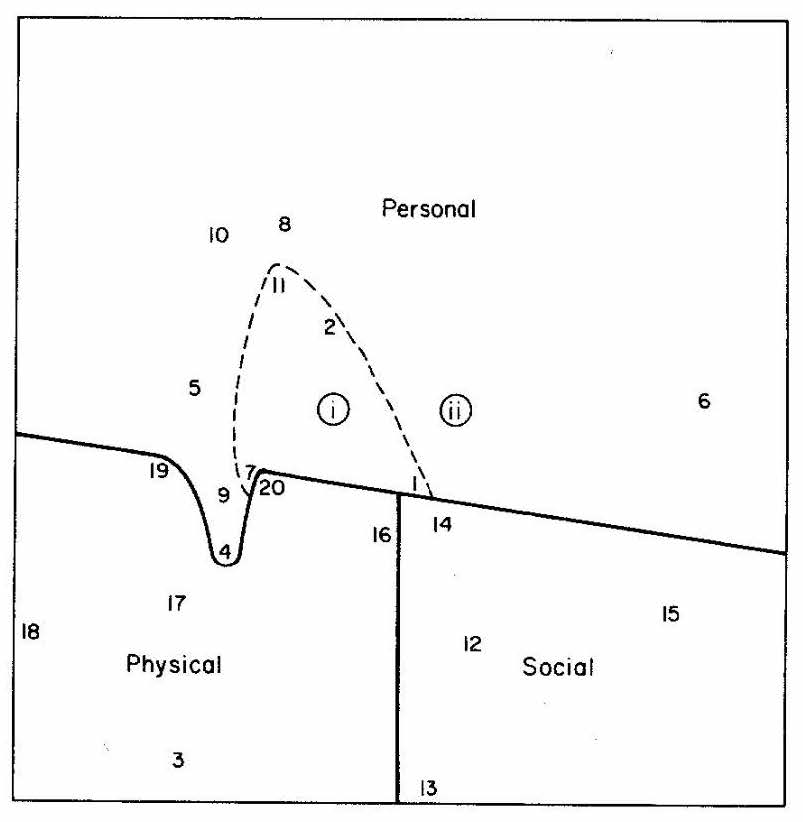
\includegraphics[width=0.45\textwidth]{figures_ref/home_regions_Sixsmith_1986}}
  \hspace*{.2in}
  \raisebox{-0.5\height}{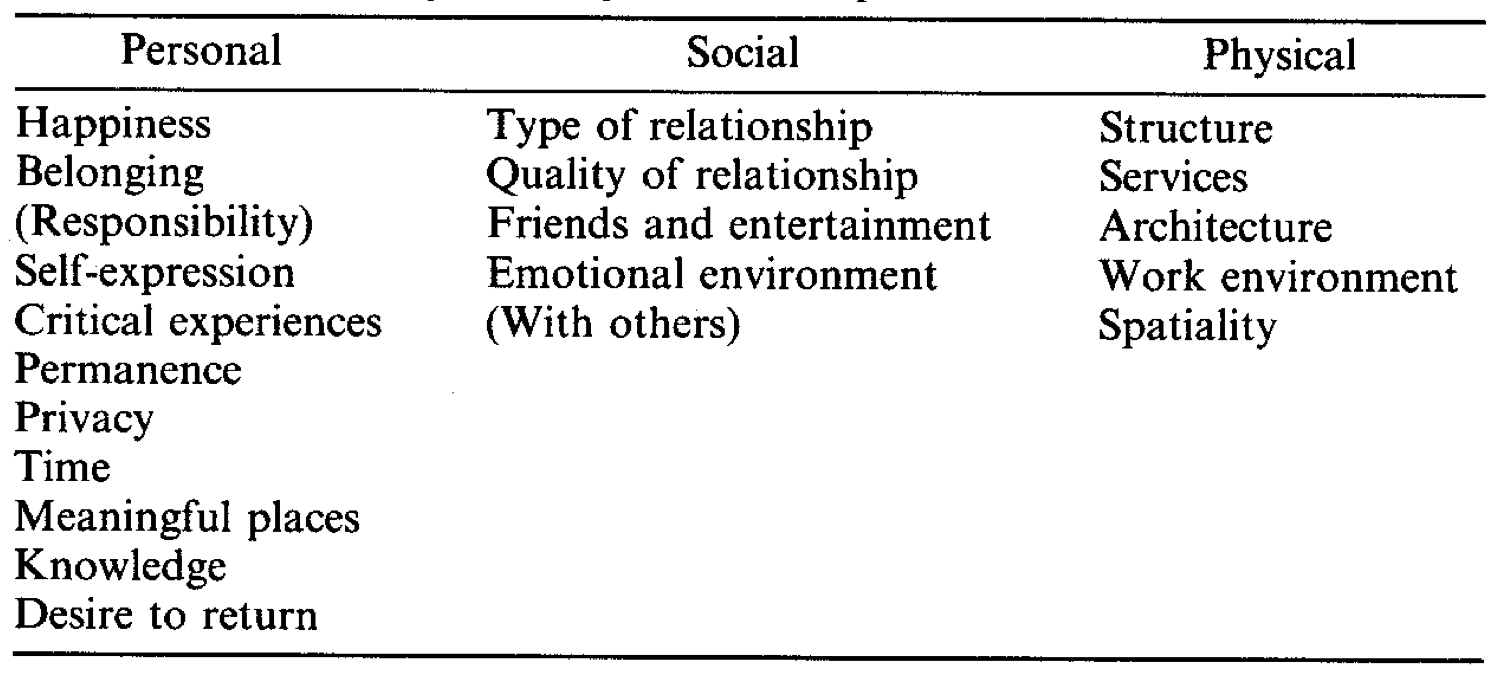
\includegraphics[width=0.45\textwidth]{figures_ref/home_categories_Sixsmith_1986}}
  \caption{The concept of home split into 3 regions (``Personal'', ``Physical'', and ``Social''). The spatial distribution of the 20 categories are yielded from Kendall's Tau correlation between the types and meanings of home defined by participants  (Adopted from \textcite{sixsmith1986meaning}).}
  \label{fig:home_regions}
\end{minipage}
\end{figure}

Culturally, the concept of home in Taiwan as a physical space has undergone changes caused by the sway of the world order \parencite{沈孟穎2015台灣現代住宅設計之轉化}. Traditionally, \textit{heyuan} houses are common architectural forms reflecting Chinese analogy of an abode to an extension of the human figure and Chinese cultures of calligraphy and sculpture. Later, influenced by Japanese power, Japanese-Western Eclectic style was introduced to Taiwan, and \zh{街屋}{jie-wu}{street house} transforms the architectural landscape by incorporating the commercial use into the residential function. This hybridization is embodied and preserved in places like Dihua Street and Dadaocheng Area.

Linguistically, \textcite{wang2005jia} have discussed the morphological development of \jia in pre-modern Chinese.

\section{Diachronic Word Embeddings}
Semantic change is a manifestation of language use in both conventional and creative ways by the language community, making textual data temporal-dependent in essence \parencite{kutuzov2018survey}. As more attention is paid to the design of diachronic corpora and digitalization of historical text, a gap bridge and rapid advancements are seen in investigating semantic change in a data-driven way, especially from a distributional semantic perspective like diachronic word embeddings \parencite{kutuzov2018survey, tahmasebi2018survey, hamilton2016law, jawahar2019contextualized}. With a growing interest in this research topic, insights have been made to highlight some key and challenging aspects of semantic change modeling \parencite{kutuzov2018survey,tahmasebi2018survey,camacho2018survey}.

% topic modeling
Besides vector space models, topic modelings are also widely applied to the study of semantic change, e.g., \acrlong{tot} \acrshort{tot} \parencite{wijaya2011understanding} and \textcite{hengchen2017phd}. In practice, probability distribution is computed for each word in the vocabulary of a specific time period, and word senses are derived from the topic distribution. For instance, the word \textit{gay} used to act as an adjective meaning happiness or cheerfulness, yet it shifts to refer to homosexuality; the word \textit{awful} comes to have less intensity and negativity in meaning, and the k-means clustering shows that words with the highest tf-idf scores do not belong to the same clusters, indicating that these words are diverse in meaning and the word \textit{awful} is then used as an adverbial intensifier with general meaning \parencite{wijaya2011understanding}; for the word \textit{mouse}, by decreasing the k in k-means, two clusters can be merged, and the last cluster represents the additional meaning acquired with the word \textit{mouse}. Therefore, Latent Dirichlet Allocation (LDA) or topic modeling accompanied by clustering method is insightful when we examine the topic density of each cluster of a given time period, top words with the highest scores by the selected metric (i.e., tf-idf scores), merging of clusters by means of adjusting the number of clusters, as well as links between words from the co-occurrence network. Ultimately, the evolution of dynamic networks, specifically temporal exponential random graph model (ERGM)\parencite{robins2007introduction} is proposed to model the network of co-occurence in a diachronic vein.

In contrast, topic models are also used to yield topics that are most common in a given time period in order to anchor words that should be evaluated for the results \parencite{antoniak2018evaluating}. By so doing, the number of topics set for the identification of anchoring words are much larger than that for \gls{tot} so that the computed mean probability is based on as diverse topics as possible.

% source data, time interval
The topic of semantic change has directed attention to the design of corpus used as input for diachronic word embeddings. In Natural Language Processing, word embeddings are commonly added to the last layer of a deep learning model to translate discrete linguistic data to continuous numeric vectors. On the other, another line of research, referred to as ``corpus-centered'' approach, focuses on the use of word embeddings as evidence for certain linguistic features or cultural characteristics \parencite{antoniak2018evaluating}. Unsupervised lexical semantic change detection refers to the task of tracing semantic change based on diachronic word embeddings trained on time-sliced textual data or (sub)corpora. The modeling rests on the assumption that change in meaning is captured if change in word co-occurrences is identified. One of the crucial steps is the collection of text and its temporal information in order to build word embeddings of different time epochs. Diachronic corpus is subject to the lack of certain documents that are difficult to survive time and thus missing, and hard to expand. The presence and absence of documents, along with a smaller or less balanced corpus, has called for techniques like bootstrapping to mitigate the issue of variability \parencite{antoniak2018evaluating}.  The division of time periods, or the granularity, is also decided in the meantime of corpora compilation. Typically, the more recent the text is created, the more refined or specific the time units are set \parencite{kutuzov2018survey}. Among the diachronic textual data currently available, the main source includes but not limited to the Google Books Ngrams Corpus\footnote{http://books.google.com/ngrams. A comprehensive review of diachronic corpora is provided by \textcite[38--41]{tahmasebi2018survey}}, Corpus of Historical American English (COHA)\footnote{\url{https://www.english-corpora.org/coha/}}, Project Gutenberg Corpus\footnote{\url{https://www.sketchengine.eu/project-gutenberg-corpus/}} and self-compiled corpora with text from newspapers and online social media. While large-scale projects have led to the release of various pre-trained word embeddings, new word embeddings continue to be trained to allow for more diversity and richness of the textual contents, and to adapt to specific research questions to be answered. This trend pertains to the definition of ``diachronic'', which highlights the characteristics of the source data with long stretch of time, and even from a long time ago in history.

Regarding conversational diachronic corpus, \parencite{giulianelli2019lexical} uses the r/LiverpoolFC corpus, which contains 40 million words from posts on the English football team Liverpool from 2011 to 2017. Each utterance is annotated with a timestamp, and the dataset includes binary annotations of change on 100 selected words by 26 r/LiverpoolFC users themselves. The compilation of this corpus is based on sufficiently high temporal granularity, enabling detection of abrupt shifts, the language use of a specific community. However, it is non-uniformly distributed, and thus it is more difficult to study changes in some of the time periods when a few user posts are generated.

\begin{table}[H]
  \centering
  \begin{tabularx}{\textwidth}{lp{7.5cm}}
    \toprule
      \multicolumn{1}{c}{Literature} &
      \multicolumn{1}{c}{Use cases} \\ %& focus \\
    \midrule
    \textcite{kulkarni2015statistically} & apple, tape \\ %& time point detection and cross-domain analysis \\
    \textcite{hamilton2016law} & gay, broadcast, awful\footnotesymbol \\ %& correlation with observed frequencies and polysemies\\
    \textcite{hamilton2016cultural} & actually, must, promise, gay, virus, cell \\ %& cultural and linguistic shift \\
    \textcite{kutuzov2017tracing} & war, peace, stable \\ % & monitoring world events\\
    \textcite{rodda2017panta} & πνεῦμα `breath' \textrightarrow\space `spirit' (Ancient Greek) \\ %& exploration in Ancient Greek \\
    \textcite{yao2018dynamic} & apple, amazon, obama, and trump \\
    \textcite{rudolph2018dynamic} & intelligence, iraq, jobs, prostitution \\
    \textcite{antoniak2018evaluating} & marijuana \\ %& word associations in different corpora \\
    \textcite{hu2019diachronic} & please, alien \\ %& contextualized embeddings with sense inventories
    \textcite{rodina2020elmo} & провальный `a place where the surface collapsed inward' or `loss of consciousness' \textrightarrow\space `failed' (Russian) \\
  \bottomrule
  \end{tabularx} \\
  \footnotesize{*See also sense shift based on earlier literature with corpus data in \textcite{hamilton2016law}}
  \caption{Example case studies from literature}
  \label{use_case}
\end{table}
% source: https://tex.stackexchange.com/questions/229289/arrow-in-text-mode
% провальный

% laws of semantic change
Diachronic word embeddings can be used to discover more possibilities of unknown change cases and underlying causes of general semantic change \parencite{hamilton2016cultural,kutuzov2017tracing,heuser2017word}. In \textcite{hamilton2016cultural}, it is concluded that linguistically-driven semantic change occur more slowly than socially-motivated phenomenon. The invention of new technologies serves as prominent examples of cultural drift, as in \textit{apple} and \textit{cell}. \textcite{kutuzov2017tracing} exemplifies how social events such as armed conflicts are traced by monitoring word associations with ``anchor words'' like \textit{war}, \textit{peace}, and \textit{stable}. Lists of words with the highest similarity scores or analogous pairs of words are analyzed to verify the results of diachronic word embeddings. In \textcite{hamilton2016cultural}, the results of linear regression shows that a local measure of this partial list is sufficient to account for the phenomenon of a cultural drift. Another example is how \textit{president} becomes closer to \textit{Obama} during his term, as well as \textit{Israel’s Prime Minister} and \textit{Christopher Nolan, The
Dark Knight, 2008} \parencite{rosin2017learning} by finding continuous peaks of lowest distance between vectors with dataset YAGO2\footnote{The latest version is released in 2020.} that contain temporal relations of named entities.

On top of that, based on the self-similarity scores of the English lexicon between 1850 and 2009, \textcite{dubossarsky2015bottom} find that lexical semantic change positively correlates with the centroid of a word's cluster, which is symbolic of the word's prototype, hence the ``law of prototypicality.'' In \textcite{xu2015computational}, near-synonyms are shown to change in parallel, and thus the law of parallel change is more favorable than the law of differentiation. The law of conformity and innovation are put forward by \textcite{hamilton2016law}; the former posits that observed frequency positively correlates with the rate of semantic change, while the latter asserts that semantic change is positively influenced by a word's polysemy, the number of a word's senses, in controlled frequency. However, different conclusions exist given different experiment settings and source data, so no consensus has been reached regarding a wider generalization of semantic change in more languages building upon diachronic word embeddings.% lexical replacement? \parencite{tahmasebi2018survey}

% embedding alignment
Additionally, if time-specific embeddings are separately trained, the embeddings are randomly initialized, and it is necessary to align them in the same vector space \parencite{hamilton2016law}. Thus, the alignment of embeddings leads to the comparability of cosine similarity scores of words from different time periods. To project separately trained word embeddings, linear transformation, distance-preserving projection, second-order embeddings that consist of vectors of word's similarities to all other words in the shared vocabulary of all models are used. The most widely adopted alignment algorithm is proposed by \textcite{hamilton2016law}, who utilizes second-order embeddings and orthogonal Procrustes transformations at the same time. Another line of research resorts to jointly learning word representations of all time periods by incrementally updating the model. Furthermore, the hierarchical softmax function is introduced to improve the efficiency of the updating.

In addition to alignment of separately trained embeddings, temporal referencing (TR) \parencite{dubossarsky2019timeforchange} is proposed to mitigate the noise issue induced by alignment. Because of alignmnet, the results, especially low-frequency words, are influenced by noises \parencite{dubossarsky2019timeforchange,dubossarsky2019timeout}. However, the lack of widely-accepted evaluation procedures have made it difficult to learn more about the noises invited by vector space aglinment \parencite{dubossarsky2019timeout}.

% evaluation data
Nonetheless, the scarcity of ground-truth test data has made it difficult to evaluate the employed approach. The rating-based and dictionary-based collection of evaluation data are met with low inter-rater agreement of recruited annotators and/or inaccessibility of sources from the time period of interest \parencite{tang2018state}. \textcite{kutuzov2020uio} reveal that the results based on the test data can be distinctively varied across different languages. In contrast, evaluation datasets for Present-Day English are available, as well as translations and crowd-sourced human-annotated datasets in Mandarin Chinese. In downstream tasks, the importance of constructing temporal-aware embeddings as input data is acknowledged in the form of domain adaptation \parencite{huang2019neural}. Temporal adaptation is introduced as a form of domain adaptation to diachronic word embeddings and proves effective in the task of document classification \parencite{huang2019neural}.  % SemEval 2015 Task 7: Diachronic Text Evaluation (Popescu and Strapparava, 2015, as cited in kutuzov2018survey).

% sense-level embeddings
Another challenge, namely the ``meaning conflation deficiency'', is brought up by \textcite{camacho2018survey}. Previously, word embedding technique is first implemented by \citeauthor{mikolov2013efficient} in \cite*{mikolov2013efficient}. The embeddings models such as \gls{cbow}, \gls{sgns}, \gls{svdppmi} are static, for only one vector is generated to represent each word type in the diachronic textual data. Word-level vector representations do not account for the context of the keyword. Therefore, two words are likely to move closer toward each other in vector space not necessarily because they become semantically closer, possibly because one of the words undergoes meaning change on the sense level. Due to the static nature of word embeddings, \textcite{hu2019diachronic} point out that the results do not show which sense has changed, and which remains stable, if not at a ``coarse-grained'' level. While static word embeddings rely on the analysis of neighboring words with the keyword to determine the presence or absence of meaning change, contextualized word embeddings mapped tokens to a possibly infinite sets of data points, allowing various methods to depict the subset of data. Pre-trained language models like ELMo and BERT are dynamic and contextualized. Multiple embeddings can be extracted to represent a word in various contexts, thus allowing different senses of a word to be distinguished. It is possible to produce mappings between contextualized word representations and sense descriptions from external linguistic resources (e.g. the Oxford English Dictionary) \parencite{hu2019diachronic}.

Notwithstanding, although context-independent and contextualized diachronic embeddings are proposed and explored in an increasing body of research to detect the presence of semantic change, which models are more capable of capturing this linguistic phenomenon remains an on-going topic that calls for evaluation methods for diachronic embeddings. It is debatable whether simpler models results in better performance \parencite{schlechtweg2019wind}. Firstly, datasets like DURel (Diachronic Usage Relatedness)\footnote{\url{https://www.ims.uni-stuttgart.de/en/research/resources/experiment-data/durel/}} are established based on human ratings \parencite{schlechtweg2018diachronic} and word injection \parencite{schlechtweg2019wind}, which is is based on similar concepts like domain-specific word sense disambiguation or term ambiguity detection, inspired by term extraction and synchronic version of SURel (Synchronic Usage Relatedness)\footnote{\url{https://www.ims.uni-stuttgart.de/en/research/resources/experiment-data/surel/}} where variation lies in sense divergence across domains for research topics like online language analysis. However, evaluation data are scarce \parencite{wevers2020digital}, hand-picked attested examples from literature or dictionaries with tags like ``obsolete'' \parencite{hamilton2016cultural} have proven that automatic semantic change detection is able to capture semantic change (See \tref{use_case}) \parencite{schlechtweg2019wind}, but results still vary depending on test or evaluation data that are currently available. The result of \textcite{schlechtweg2019wind} shows that \gls{sgns} with orthogonal Procrustes alignment achieves the highest performance based on the DURel dataset, whereas topic modeling has the least correlation with the examined dataset. Furthermore, the results in \textcite{schlechtweg2019wind,dubossarsky2017outta} shows that cosine distance (global neighborhood distance) outperforms local neighborhood distance under the condition of aligned embeddings, and the results of topic modeling is sensitive to corpus size and frequency of the target words, which make it a less desirable method in this study, as pre-modern Chinese texts might not reflect accurate counts of types and tokens.

%The BERT pre-trained language model can be used in company with sense inventories or cluster analysis. Using the BERT pre-trained language model, \textcite{hu2019diachronic} track the evolution of 4881 English words from 1810 to 2009 in the Corpus of Historical American English (COHA), and visualizes the interactions of words' senses. The source texts from COHA are concordance lines which contain target words with a frequency of at least 10 times for over 50 consecutive years. Additionally, the sense identification task is performed by using example sentences in the Oxford English Dictionary (OED) as the knowledge base for similarity comparison with texts from COHA, and the total number of senses from the OED is 15836. Firstly, the last hidden layer of a target word's embedding is extracted from the pre-trained BERT language model. This token embedding is then compared with each sense representation retrieved from the OED word entry to determine which sense the target word belongs to. In \textcite{giulianelli2019lexical}, the target words are collected from \textcite{gulordava2011distributional} with annotated data on judgement task. Then, their cluster analysis reveals that types of semantic change can be identified, e.g., literal/metaphorical meanings, different senses of a polysemous word, words with different syntactic categories, and affixation. It is concluded that the change in sense distribution follows the ``S shape'' proposed in linguistics. Moreover, the actual uses of a certain sense can be inspected from the collected data. Their method is shown to be effective on detection of short-term community-specific changes in word usages by including football data as the conversational corpus compared to diachronic corpus in their study. Their subsequent work is expanded to more languages and judgement data in the SemEval 2020 task \parencite{kutuzov2020uio}.

Instead of sense inventories, various clustering algorithms are resorted to induce senses of target words, including K-Means, Gaussian mixture models \parencite{giulianelli2019lexical}.

% integration of other approaches
In comparison with other approaches of semantic change detection, diachronic word embeddings exhibit a stronger explanatory power than frequency-based methodologies such as raw and relative frequency counts, collocational analysis \parencite{kutuzov2018survey}. Indeed, it is convenient to manipulate word vectors, but past literature also presents the results and analysis in combination of the above two or more approaches to generalize the underlying principles of semantic change or echo with the proposed linguistic hypotheses \parencite{tahmasebi2018survey}.% word sense induction, word sense disambiguiation, novel sense detection

The compilation of corpora to include historical texts and annotations enables more detailed linguistic analysis. Examples include
the Corpus of Historical American English (COHA, 1810-2000)\footnote{https://www.english-corpora.org/coha/}, 
A Representative Corpus of Historical English Registers (ARCHER, 1600-1999)\footnote{https://www.projects.alc.manchester.ac.uk/archer/}
Royal Society Corpus (RSC, 1665-1996)\footnote{https://fedora.clarin-d.uni-saarland.de/rsc/}, 
Corpus of Late Modern English Texts (CLMET, 1710-1920)\footnote{https://perswww.kuleuven.be/~u0044428/}, 
Hansard Corpus (1803-2005)\footnote{https://www.english-corpora.org/hansard/}, among many others.

In Chinese, the number of diachronic corpora is relatively scarce, including Sheffield Corpus of Chinese\footnote{https://www.dhi.ac.uk/scc/} and Academia Sinica Ancient Chinese Corpus (中央研究院古漢語語料庫, hereafter ASAC Corpus)\footnote{http://lingcorpus.iis.sinica.edu.tw/early/} \parencite{wei1997corpus}. The ASAC Corpus is divided into 3 sub-corpora based on the development of Chinese syntax, namely Old Chinese subcorpus (上古 from pre-Qing to pre-Han), Middle Chinese subcorpus (中古 from Late Han to the Six Dynasties), and Early Mandarin Chinese subcorpus (近代 from Tang to Qing) to offer a synchronic sketch and a basis for diachronic comparisons. In the Academia Sinica Tagged Corpus of Early Mandarin Chinese (中央研究院近代漢語語料庫), raw texts are available from the Western Han dynasty to the Pre-Qing dynasty, with part of the texts imported from Scripta Sinica (漢籍全文資料庫計畫). It is believed that corpora creation is the foundation for a more thorough and accurate depiction for data collection during the establishment of lexical databases.



\section{Visualizing semantic change}
In view of the scale of data, semantic change modeling is evaluated on two grounds--the combination of statistical testing and visualizations, as well as classification tasks \parencite{tang2018state}. In addition to the exploration of linear relationships such as word analogies, high-dimensional visualization techniques are employed to assess the results of word representation learning \parencite{liu2017visual}. Visualization of diachronic data allows researchers to explore any target word to see how the data changes along with time.

To visualize the results, vectors originally trained in high-dimensional space are transformed and projected in two or three dimensions. \gls{pca} and \gls{tsne} \parencite{vandermaaten2008tsne} are two common methods of dimensionality reduction. Only the most influential dimensions are retained using the former approach, while the latter reflects more geometrical structure of the high-dimensional data. However, the exploration of the internal structure and properties of an embedding is generally non-interactive \parencite{smilkov2016projector}. In \cite*{smilkov2016projector}, Google releases the Embedding Projector under the TensorBoard framework, which provides users with many interactive functionalities such as zooming, filtering, inspection of data points with metadata created in the table format by users \parencite{smilkov2016projector}.

\textcite{coenen2019visualizing} recognizes the adaptability of BERT to various downstream tasks and the possibility of the language model to extract useful features from raw textual data. To understand the internal structure of BERT and how discrete linguistic units are translated into continuous numeric vectors, \textcite{coenen2019visualizing} use UMAP visualization of the token vectors and nearest-neighbor classifier. Semantically, fine-grained sense information is encoded in BERT, even in low-dimensional subspace. \textcite{coenen2019visualizing} conclude that both semantic and syntactic information are encoded in the contextualized embeddings in ``complementary subspaces.'' Yet, an attention-based model like BERT does not necessarily ``respect semantic boundaries when attending to neighboring tokens, but rather indiscriminately absorb meaning from all neighbors.'' \parencite{coenen2019visualizing}

It is summarized in \textcite{tang2018state} that the novelty of a sense can be understood as the change in sense distribution of different time intervals. The diachornic sense distribution can be visualized based on both word-level and sense-level embeddings \parencite{dubossarsky2015bottom,hu2019diachronic}. In \textcite{dubossarsky2015bottom}, the distance of a word's centroid is pinpointed to find out the emergence of new senses. A trajectory of sense evolution is graphically represented in \textcite{hu2019diachronic}. The rise of a new sense can be depicted in company with other senses in a competitive or cooperative relationship. Also \parencite{gonen2020simple}.

However, the division of time periods, or the granularity, examined in previous studies, especially those on laws of semantic change, is restricted to the nineteenth century onward. Additionally, to trace semantic change of pre-modern Chinese, we need to account for the disyllabic development of words. Therefore, we aim to analyze both pre-modern and modern Chinese texts, which would be the first attempt to apply both computational and statistical
models to explore the interplay between disyllabic development of words and semantic change in Chinese.

\end{document}

% conferences:
% SemEval
% NLP for semantic change (https://semanticshifts.sciencesconf.org/data/pages/Course12.pdf)
% https://driftselection-evolang2020.github.io/#submission_(ended)